\chapter{Implementazione e prove sperimentali}

In questo capitolo verranno presentate le caratteristiche tecnologiche dei veicoli utilizzati nella fase sperimentale, le proprietà fisiche di ogni scenario modellato e le varie misure di qualità.

Per ogni scenario verrà illustrata la complessità ambientale, insieme alla rappresentazione reale ed al modello della relativa mappa, per comprendere le caratteristiche morfologiche dell'area e la strattura degli ostacoli presenti.
Verranno, inoltre, analizzate le informazioni relative ai parametri utilizzati nella fase di ottimizzazione e adattamento delle metaeuristiche alla missione.
 
Infine, i risultati sperimentali verranno presentati alla fine di ogni scenario ed alla fine del capitolo per un'analisi comparative con risultati già presenti in letteratura.

\section{Specifiche tecniche del drone}

Le caratteristiche ambientali dei vari scenari sono state prese in considerazione per le specifiche tecniche degli UAV disponibili in commercio. 
La tecnologia selezionata per modellare gli agenti responasbili del completamento della missione è la seguente:
\begin{itemize}
    \item \textit{Modello drone:} Dji Matrice M200
    \item \textit{Sensore di rilevamento:} Dji Zenmuse XT2 (Visual + Thermal Camera) 
\end{itemize}
Tale tecnologia è stata adottata sulla base delle conoscenze e delle competenze acquisite in diversi progetti che utilizzano la tecnologia UAV per il monitoraggio e la sorveglianza ambientale. 
In particolare, la tecnologia di rilevamento proposta, si basa su \cite{persechino2010aerospace} e \cite{lega2012using};

\begin{figure}[H] 
    \captionsetup{justification=centering, margin=2cm, font=footnotesize}
    \begin{center}
    \makebox[\textwidth]{\includegraphics[width=0.4\paperwidth]{img/dji_matrice_sensore.jpg}}
    \end{center}
    \caption{Rappresentazione del drone Dji Matrice M200 equipaggiato con il sensore Dji Zenmuse XT2.}
    \label{dji_matrice}
\end{figure}

Le tabelle \ref{tabella_tecnologia_drone} e \ref{tabella_tecnologia_sensore}, invece, mostrano, rispettivamente, la configurazione parametrica relativa alle specifiche del drone  \cite{matrice200} e le apparecchiature di sensing utilizzate in fase di simulazione.

\begin{table}[H]
    \centering
    
    \begin{tabular}{|l|c|}
    \hline
    \textbf{Parameter}              & \textbf{Value}                \\ \hline
    Radius                          & $0.3 \; m$                    \\ \hline
    Max speed                       & $17 \; m/s$                   \\ \hline
    Max acceleration                & $4.4 \; m/s^{2}$              \\ \hline
    Max angular speed               & $2.6 \; rad/s$                \\ \hline
    Max angular acceleration        & $7 \; rad/s^{2}$              \\ \hline
    Battery duration                & $24 \; min$                   \\ \hline
    Obstacle vision distance        & $3-30 \; m$                   \\ \hline
    Obstacle vision angle           & $60 \; \circ$                     \\ \hline
    \end{tabular}%
    
    \caption{Specifiche tecniche del modello di drone \textit{Dji Matrice 200}.}
    \label{tabella_tecnologia_drone}
\end{table}

\begin{table}[H]
    \centering
    
    \begin{tabular}{|c|c|c|}
    \hline
    \begin{tabular}[c]{@{}l@{}}\textbf{Sensing} \\ \textbf{technology}\end{tabular}                   & \textbf{Sensor model}                 & \begin{tabular}[c]{@{}l@{}}\textbf{Sensing} \\ \textbf{radius}\end{tabular}        \\ \hline
    \begin{tabular}[c]{@{}l@{}}Visual + \\ Thermal\end{tabular}                              & Dji Zenmuse XT2                       & 5 m                            \\ \hline    
    \end{tabular}%    
    \caption{Specifiche tecniche dell'equipaggiamento di sensing.}
    \label{tabella_tecnologia_sensore}
\end{table}

\section{Scenario \textit{Illegal Dump}}

In questa sezione sono illustrati lo scenario utilizzato e le varie misure di qualità. 
Lo scenario è statico: \textit{Illegal Dump} si basa sulla mappa di una discarica abusiva di Paternò, Italia \cite{trashout2018}.
Di seguito sono riportate le caratteristiche dello scenario:

\begin{itemize}
    \item \textit{Area in metri:} 400 x 400
    \item \textit{Area in patch:} 201 x 201
    \item \textit{Dimensione patch:} 1.99m x 1.99m
    \item \textit{Conversione spaziale:} 1 m = 0.502 patch
    \item \textit{Conversione temporale:} 1 s = 1 tick
    \item \textit{Numero target presenti nell'area:} 42
    \item \textit{Numero ostacoli presenti nell'area:} 7174
    \item \textit{Flotta utilizzata:} 80 droni
\end{itemize}

La configurazione dei parametri utilizzata nella fase sperimentale dello scenario \textit{Illegal Dump} è illustrata nella tabella di seguito.

\begin{table}[H]
    \centering
    
    \begin{tabular}{|l|c|}
    \hline
    \textbf{Parameter}              & \textbf{Value}                \\ \hline
    Radius                          & $0.3 \; m$                    \\ \hline
    Max speed                       & $17 \; m/s$                   \\ \hline
    Max acceleration                & $4.4 \; m/s^{2}$              \\ \hline
    Max angular speed               & $2.6 \; rad/s$                \\ \hline
    Max angular acceleration        & $7 \; rad/s^{2}$              \\ \hline
    Battery duration                & $24 \; min$                   \\ \hline
    Obstacle vision distance        & $3-30 \; m$                   \\ \hline
    Obstacle vision angle           & $60 \; \circ$                     \\ \hline
    \end{tabular}%
    
    \caption{Configurazione parametrica per la fase sperimentale dello scenario \textit{Illegal Dump}.}
    \label{tabella_costanti_dump}
\end{table}

\begin{table}[H]
    \centering
    
    \begin{tabular}{|l|c|c|c|}
    \hline
    \textbf{Scenario}              & \textbf{Area size (m x m)}     & \textbf{Area size (patch x patch)}      \\ \hline
    Illegal Dump                   & 400 x 400                      & 201 x 201                           \\ \hline
    \end{tabular}%
    
    \caption{Caratteristiche dello scenario Illegal Dump.}
    \label{tabella_scenario}
\end{table}

Per osservarne la complessità ambientale, le figure \ref{dump_map} e \ref{dump_scenario} mostrano la mappa satellitare utilizzata per \textit{Illegal Dump}, e la corrispondente immagine vettoriale iniziale rappresentata nell'ambiente di simulazione, rispettivamente. 
Qui, gli ostacoli (edifici e alberi) sono rappresentati in nero, mentre i bersagli sono rappresentati come punti rossi. 
I droni, rappresentati come triangoli viola, sono posizionati agli angoli e sono orientati verso il centro dell'area.

\begin{figure}[H] 
    \captionsetup{justification=centering, margin=2cm, font=footnotesize}
    \begin{center}
    \makebox[\textwidth]{\includegraphics[width=0.3\paperwidth]{img/dump_map.png}}
    \end{center}
    \caption{Immagine satellitare dello scenario Illegal Dump.}
    \label{dump_map}
\end{figure}

\begin{figure}[H] 
    \captionsetup{justification=centering, margin=2cm, font=footnotesize}
    \begin{center}
    \makebox[\textwidth]{\includegraphics[width=0.3\paperwidth]{img/dump_scenario.png}}
    \end{center}
    \caption{Immagine vettoriale dello scenario Illegal Dump.}
    \label{dump_scenario}
\end{figure}

\section{Risultati sperimentali}

Informazioni esperimento:
\begin{itemize}
    \item Algoritmo: Artificial Bee Colony (ABC)
    \item Dimensione vettore parametri: $D = 9$
    \item Numero individui per popolazione: $NP = 4\cdot D = 36$
    \item Fattore di amplificazione: $F = 0.7$
    \item Costante di Crossover: $CR = 0.7$
    \item Strategia di Crossover: \textit{DE/best/1/bin}
\end{itemize}

\begin{figure}[H] 
    \captionsetup{justification=centering, margin=2cm, font=footnotesize}
    \begin{center}
        \makebox[0.5\paperwidth]{
            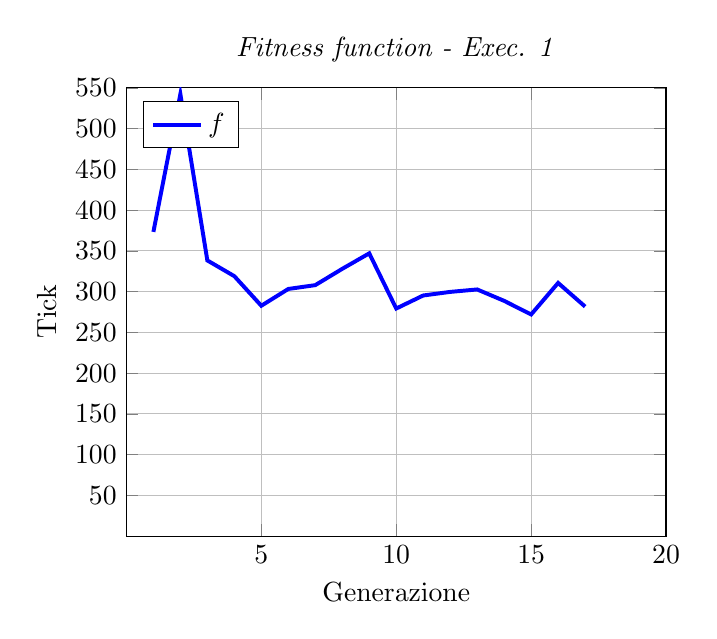
\begin{tikzpicture}
                \begin{axis}[
                    title={\textit{Fitness function - Exec. 1}},
                    xlabel={Generazione},
                    ylabel={Tick},
                    xmin=0, xmax=20,
                    ymin=0, ymax=550,
                    xtick={5,10,15,20},
                    ytick={50,100,150,200,250,300,350,400,450,500,550},
                    legend pos=north west,
                    grid=major,
                    %ymajorgrids=true,
                    %xmajorgrids=true
                    %grid style=dashed,
                ]
                
                \addplot[
                    color=blue,
                    line width=0.5mm,
                    ]
                    coordinates {
                        (1,373.3)(2,542.3)(3,338.3)(4,319.0)(5,282.7)(6,303.3)(7,308.0)(8,328.0)(9,347.0)(10,279.3)(11,295.3)(12,299.7)(13,302.7)(14,288.7)(15,272.0)(16,310.7)(17,281.7)
                    };
                    \legend{$f$}
                
                \end{axis}
            \end{tikzpicture}
        }
    \end{center}
    \caption{Andamento della funzione obiettivo al variare di generazione.}
    \label{modello3d_feromone}
\end{figure}   

\begin{figure}[H] 
    \captionsetup{justification=centering, margin=2cm, font=footnotesize}
    \begin{center}
        \makebox[0.5\paperwidth]{
            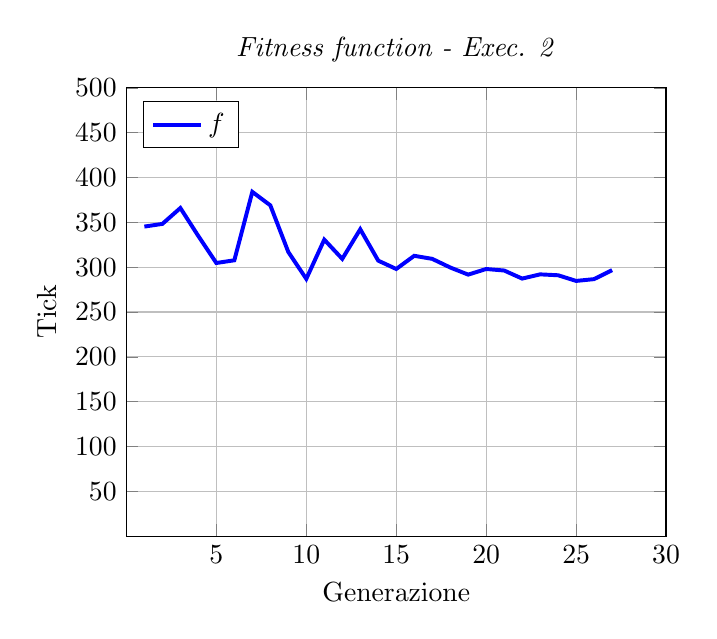
\begin{tikzpicture}
                \begin{axis}[
                    title={\textit{Fitness function - Exec. 2}},
                    xlabel={Generazione},
                    ylabel={Tick},
                    xmin=0, xmax=30,
                    ymin=0, ymax=500,
                    xtick={5,10,15,20,25,30},
                    ytick={50,100,150,200,250,300,350,400,450,500},
                    legend pos=north west,
                    grid=major,
                    %ymajorgrids=true,
                    %xmajorgrids=true
                    %grid style=dashed,
                ]
                
                \addplot[
                    color=blue,
                    line width=0.5mm,
                    ]
                    coordinates {
                        (1,345.3)(2,348.3)(3,366.0)(4,334.7)(5,304.7)(6,307.7)(7,384.0)(8,369.0)(9,317.0)(10,287.0)(11,330.7)(12,309.3)(13,342.3)(14,307.3)(15,298.0)(16,312.7)(17,309.3)(18,299.7)(19,291.7)(20,298.0)(21,296.3)(22,287.3)(23,292.0)(24,291.0)(25,284.7)(26,286.7)(27,296.7)
                    };
                    \legend{$f$}
                
                \end{axis}
            \end{tikzpicture}
        }
    \end{center}
    \caption{Andamento della funzione obiettivo al variare di generazione.}
    \label{modello3d_feromone}
\end{figure}   

\begin{figure}[H] 
    \captionsetup{justification=centering, margin=2cm, font=footnotesize}
    \begin{center}
        \makebox[0.5\paperwidth]{
            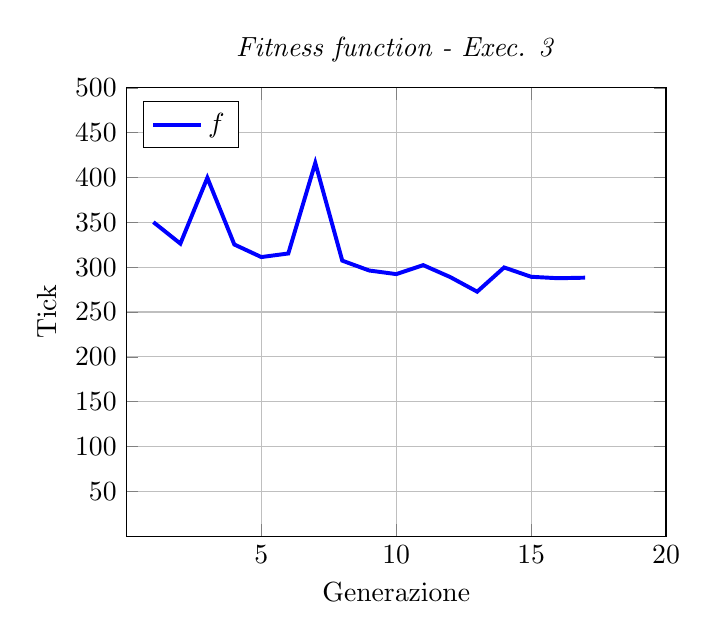
\begin{tikzpicture}
                \begin{axis}[
                    title={\textit{Fitness function - Exec. 3}},
                    xlabel={Generazione},
                    ylabel={Tick},
                    xmin=0, xmax=20,
                    ymin=0, ymax=500,
                    xtick={5,10,15,20},
                    ytick={50,100,150,200,250,300,350,400,450,500},
                    legend pos=north west,
                    grid=major,
                    %ymajorgrids=true,
                    %xmajorgrids=true
                    %grid style=dashed,
                ]
                
                \addplot[
                    color=blue,
                    line width=0.5mm,
                    ]
                    coordinates {
                        (1,350.3)(2,326.3)(3,399.7)(4,325.3)(5,311.3)(6,315.3)(7,416.3)(8,307.3)(9,296.3)(10,292.3)(11,302.3)(12,289.0)(13,272.7)(14,299.7)(15,289.3)(16,287.7)(17,288.3)
                    };
                    \legend{$f$}
                
                \end{axis}
            \end{tikzpicture}
        }
    \end{center}
    \caption{Andamento della funzione obiettivo al variare di generazione.}
    \label{modello3d_feromone}
\end{figure}  